\documentclass[11pt,a4paper]{article}

\usepackage[T1]{fontenc}
\usepackage[utf8]{inputenc}
\usepackage{lmodern}
\usepackage[margin=2.5cm]{geometry}
\usepackage{amsmath,amssymb}
\usepackage{booktabs,tabularx,array}
\usepackage{microtype}
\usepackage{xcolor}
\usepackage{listings}
\usepackage{tikz}
\usetikzlibrary{arrows.meta,positioning,fit}
\usepackage{hyperref}

\hypersetup{colorlinks=true,linkcolor=blue!50!black,citecolor=blue!50!black,urlcolor=blue!50!black}
\lstset{basicstyle=\ttfamily\small,breaklines=true,frame=single,columns=fullflexible}
\setlength{\parskip}{0.5em}
\setlength{\parindent}{0pt}

\title{Open-Domain Question Answering:\\From Lexical Retrieval to RAG\\[0.3em]
\large NLP (CS60075) Assignment II, Project 10 -- Natural Questions (Open)}
\author{Saksham Kumar (24CS10029)}

\begin{document}
\maketitle

\begin{abstract}
This report describes three open-domain question answering systems evaluated on a fixed sample of 300 questions from Natural Questions (Open), over a Wikipedia-paragraph index of 45,029 passages built for this project. Task~1 is a classical pipeline using BM25 retrieval and rule-based answer extraction. Task~2 reproduces the retrieve-then-generate design of Retrieval-Augmented Generation (RAG) using a MiniLM dense retriever and the Qwen2.5-1.5B-Instruct generator. Task~3 fuses both rankings with Reciprocal Rank Fusion (RRF) and adds a lexical groundedness check. The dense RAG system performed best, with 27.7\% Exact Match (EM) and 68.7\% recall@10. The hybrid system did not improve on it, reaching 25.7\% EM and 62.7\% recall@10. The classical system retrieved the answer within the top 10 passages for 56.7\% of questions, but achieved only 0.3\% EM. The groundedness check flagged 26 answers, none of which exactly matched a gold answer, but it caught just 11.7\% of answers scored as wrong, and some of its flags were on answers that were right in meaning. We analyse why fusion did not help and why vocabulary overlap is a weak signal of correctness.
\end{abstract}

\section{Introduction}

Open-domain question answering (QA) requires a system to answer a question using a large document collection instead of a single passage supplied with the question. The problem has two parts: \emph{retrieval}, which finds relevant evidence, and \emph{answering}, which produces a short answer from that evidence. Chen et al.'s DrQA~\cite{drqa} established this retrieve-then-read design over Wikipedia, combining a TF-IDF document retriever with a neural span reader. It serves as the conceptual starting point for this project.

The three tasks vary each part in turn:
\begin{itemize}
    \item \textbf{Task 1} uses lexical retrieval and extractive answering, with no neural components.
    \item \textbf{Task 2} uses dense retrieval and a generative language model.
    \item \textbf{Task 3} fuses the lexical and dense rankings, and uses lexical overlap as a groundedness check on generated answers.
\end{itemize}

Figure~\ref{fig:pipeline} shows how the components relate. All three systems share one passage index, one question sample, and one evaluation code path, so differences between them come from the methods and not from the data.

\begin{figure}[ht]
\centering
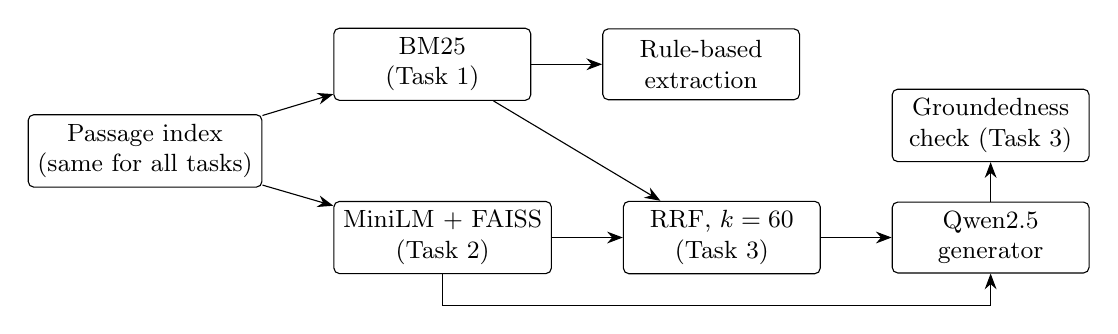
\begin{tikzpicture}[
    box/.style={draw,rounded corners=2pt,align=center,minimum height=9mm,minimum width=25mm,font=\small},
    arr/.style={-{Stealth[length=2mm]}},
    node distance=6mm and 9mm]
    \node[box] (index) {Passage index\\(same for all tasks)};
    \node[box,right=of index,yshift=11mm] (bm25) {BM25\\(Task 1)};
    \node[box,right=of index,yshift=-11mm] (dense) {MiniLM + FAISS\\(Task 2)};
    \node[box,right=of bm25] (extract) {Rule-based\\extraction};
    \node[box,right=of dense] (rrf) {RRF, $k=60$\\(Task 3)};
    \node[box,right=of rrf,yshift=0mm] (qwen) {Qwen2.5\\generator};
    \node[box,above=of qwen,yshift=-1mm] (ground) {Groundedness\\check (Task 3)};
    \draw[arr] (index) -- (bm25);
    \draw[arr] (index) -- (dense);
    \draw[arr] (bm25) -- (extract);
    \draw[arr] (bm25) -- (rrf);
    \draw[arr] (dense) -- (rrf);
    \draw[arr] (dense.south) -- ++(0,-4mm) -| (qwen.south);
    \draw[arr] (rrf) -- (qwen);
    \draw[arr] (qwen) -- (ground);
\end{tikzpicture}
\caption{The three systems. Task~2 passes dense results directly to the generator, while Task~3 passes it the fused ranking.}
\label{fig:pipeline}
\end{figure}

\section{Dataset and Passage Index}

\subsection{Question sample}
We used \texttt{google-research-datasets/nq\_open}, the open-domain variant of Natural Questions~\cite{nq,orqa}, in which each question has one or more acceptable short answers and no supplied passage. As the assignment specifies, we drew a fixed sample of $n=300$ questions from the validation split, using \texttt{numpy.random.RandomState(42)} and sampling without replacement. The seed is 42 throughout. We used no training examples, so generation is zero-shot and no model was trained or fine-tuned.

\subsection{Index construction}
Natural Questions has no passage collection of its own, so we built one from English Wikipedia using the live MediaWiki API (\texttt{prepare\_index.py}). The index is built once, then reused unchanged for all three tasks.

\textbf{Page selection.} Each question is searched twice, and the top three pages are kept from each search: once using the question as written, and once using its keywords joined with \texttt{OR}. Keywords are the question's lowercase word tokens after removing scikit-learn's English stopword list. The second query helps find pages worded differently from the question. A further 300 randomly chosen non-redirect pages act as distractors that the retrievers must filter out. \textbf{Gold answers are never used to select pages or write passages}; they are read only after the index is written, to compute a coverage statistic.

\textbf{Segmentation.} Plain-text page extracts are split into passages of about 100--200 words without crossing section boundaries:
\begin{enumerate}
    \item Sections titled References, External links, See also, Further reading, Notes, Bibliography, Sources, Citations, Footnotes, or Works cited are skipped, including their subsections.
    \item Lines are accumulated until a block reaches at least 100 words, or a section ends.
    \item Blocks over 200 words are split at sentence boundaries, and any single sentence over 200 words is cut outright.
    \item Chunks shorter than 30 words are dropped. Section-final chunks of 30--99 words are kept, so a minority of passages fall below the nominal 100-word minimum.
\end{enumerate}

\textbf{Reliability and reproducibility.} Every API response is cached on disk so that an interrupted build can resume. Requests are spaced 1~s apart and retried up to eight times with exponential backoff, following the server's \texttt{Retry-After} header when present, because the shared cluster IP address received HTTP~429 responses. Because Wikipedia changes and distractor pages are random, a rebuild would produce a different index. Reported results therefore apply to this frozen index file, whose build details are recorded in an accompanying manifest.

\textbf{Index statistics.} Table~\ref{tab:index} summarises the index, built on 31 October 2026. Answer coverage is the share of sampled questions with a gold answer appearing anywhere in the index, and so is the upper limit on recall@$k$ for any retriever. It is 86.3\%, meaning that for 41 of the 300 questions no retriever could find a gold answer string.

\begin{table}[ht]
\centering
\begin{tabular}{@{}lr@{}}
\toprule
Statistic & Value \\
\midrule
Pages selected from question searches & 1,552 \\
Random distractor pages & 300 \\
Total pages & 1,852 \\
Total passages & 45,029 \\
Answer coverage & 86.3\% (259 of 300) \\
\bottomrule
\end{tabular}
\caption{Statistics of the frozen index, from its build manifest.}
\label{tab:index}
\end{table}

\section{Evaluation Metrics}

All answers and gold strings are normalised in the SQuAD style~\cite{squad}: lowercasing, then removing punctuation and the articles \emph{a}, \emph{an}, \emph{the}, then collapsing whitespace. With several acceptable answers, the best-scoring one counts.

\textbf{Exact Match (EM)} is 1 when the normalised prediction equals any normalised gold answer, and 0 otherwise.

\textbf{Token F1} is the harmonic mean of token precision and recall, computed on token multisets:
\begin{equation}
    P = \frac{|T_{\text{pred}} \cap T_{\text{gold}}|}{|T_{\text{pred}}|},\quad
    R = \frac{|T_{\text{pred}} \cap T_{\text{gold}}|}{|T_{\text{gold}}|},\quad
    F_1 = \frac{2PR}{P+R}.
\end{equation}

\textbf{Recall@$k$} is the fraction of questions where a normalised gold answer appears as whole words in at least one of the top $k$ passages, for $k \in \{1,3,5,10\}$. Whole-word matching stops ``no'' from matching inside ``know''. Natural Questions provides no gold passages, so this is a string-presence measure: a passage can contain the answer string without actually supporting the answer, which makes recall@$k$ somewhat optimistic, particularly for short answers.

\textbf{Groundedness metrics} are defined in Section~\ref{sec:groundedness}.

\section{Task 1: Classical Lexical Retrieve-and-Extract}

\subsection{BM25 retrieval}
BM25~\cite{bm25} scores a passage $d$ for query $q$ by summing, over the query terms, an inverse document frequency weight multiplied by a saturating term-frequency component:
\begin{equation}
    \text{BM25}(q,d) = \sum_{t \in q} \text{IDF}(t)\,
    \frac{f(t,d)\,(k_1+1)}{f(t,d) + k_1\left(1 - b + b\frac{|d|}{\text{avgdl}}\right)}.
\end{equation}
Rare terms therefore count for more, repeated terms give diminishing returns, and long passages are penalised. We used \texttt{rank\_bm25.BM25Okapi} with $k_1=1.5$ and $b=0.75$, as specified. Passages and queries are tokenized with \texttt{text.lower().split()}.

We also tested a stricter tokenizer that split on punctuation and removed stopwords, on the hypothesis that attached punctuation was preventing matches. It produced worse results on the 300-question rerun, so it was discarded. All results in this report use the original whitespace tokenizer.

\subsection{Rule-based answer extraction}
Answers are taken only from the top-ranked passage, in two steps:
\begin{enumerate}
    \item \textbf{Sentence selection.} spaCy's \texttt{en\_core\_web\_sm} model splits the passage into sentences. The sentence sharing the most normalised word types with the question is selected, and the earliest such sentence wins ties.
    \item \textbf{Span selection.} The answer is the longest span, by character count, among the sentence's noun chunks and its \texttt{CARDINAL} or \texttt{DATE} entities. If none exists, the whole sentence is returned.
\end{enumerate}

\section{Task 2: Retrieval-Augmented Generation}

\subsection{The paper: Lewis et al.\ (2020)}
RAG~\cite{rag} addresses a limitation of large language models: their factual knowledge is stored implicitly in their parameters, which makes it hard to inspect, trace to a source, or update. RAG pairs a \emph{parametric} sequence-to-sequence generator with a \emph{non-parametric} retrievable document index, and trains them as one probabilistic model.

\textbf{Retriever.} RAG uses Dense Passage Retrieval (DPR)~\cite{dpr}, a bi-encoder with separate BERT-based question and passage encoders. A passage's retrieval score is the inner product of the two embeddings:
\begin{equation}
    p_\eta(z \mid x) \propto \exp\left(\mathbf{d}(z)^\top \mathbf{q}(x)\right).
\end{equation}
Because both sides become vectors, a passage can rank highly while sharing few exact words with the question. The paper's knowledge source is a December 2018 Wikipedia dump split into disjoint 100-word chunks, about 21 million documents, indexed with FAISS~\cite{faiss} using a Hierarchical Navigable Small World approximation.

\textbf{Generator.} The generator is BART, a pretrained sequence-to-sequence model. The question and retrieved passage are concatenated as its input.

\textbf{Marginalisation.} RAG treats the retrieved document as a latent variable and marginalises over the top $k$ documents:
\begin{equation}
    p(y \mid x) \approx \sum_{z \in \text{top-}k} p_\eta(z \mid x)\, p_\theta(y \mid x, z).
\end{equation}
The paper's two variants differ in where this happens. \textbf{RAG-Sequence} uses one document for a whole answer and marginalises over complete hypotheses, while \textbf{RAG-Token} can draw on a different document for each generated token. Training minimises the negative marginal log-likelihood by gradient descent, with no explicit document labels, and updates the query encoder and generator; the document encoder and index stay fixed.

\textbf{Reported results.} On Natural Questions, RAG reached 44.1\% (Token) and 44.5\% (Sequence) EM, above DPR's extractive reader at 41.5\% and closed-book T5 at 34.5\%~\cite{rag}. The paper also notes that generation can draw on documents that contain clues without stating the answer verbatim, which purely extractive approaches cannot use. Knowledge can also be updated by swapping the index, without retraining.

\subsection{Our implementation}

\textbf{Dense retrieval.} Passages are embedded with \texttt{sentence-transformers/all-MiniLM-L6-v2}~\cite{sbert}, in batches of 64, and $\ell_2$-normalised. They are stored in a FAISS \texttt{IndexFlatIP} index, so inner product equals cosine similarity and search is exact. Questions are embedded the same way at query time.

\textbf{Generation.} We used \texttt{Qwen/Qwen2.5-1.5B-Instruct}~\cite{qwen}, an open instruction-tuned model, in 16-bit precision on GPU. The top five passages are each truncated to 200 tokens and inserted into a prompt formatted with the model's chat template:

\begin{lstlisting}
Answer the question based strictly on the provided context. Reply with only
the answer as a short phrase, not a full sentence. If it is a yes/no question,
reply with only yes or no.

Context:
Passage 1: ...
...
Passage 5: ...

Question: {question}
\end{lstlisting}

The short-answer instruction exists because EM rewards only the exact answer string, and a correct full sentence scores zero. Generation uses at most 64 new tokens with greedy decoding (\texttt{do\_sample=False}), which is the deterministic equivalent of the specified temperature of 0. Only the newly generated tokens are decoded and scored.

\subsection{Differences from the paper}
Table~\ref{tab:rag-diff} summarises how our implementation differs from RAG. The assignment prescribes the retriever and generator family, and these choices also fit the available compute. Conceptually, our system is a \emph{retrieve-then-generate pipeline}, sometimes called ``RAG-style'', not RAG's jointly trained latent-variable model.

\begin{table}[ht]
\centering
\small
\begin{tabularx}{\textwidth}{@{}lXX@{}}
\toprule
Aspect & Lewis et al.~\cite{rag} & This project \\
\midrule
Retriever & DPR bi-encoder & MiniLM-L6-v2, 384-dimensional embeddings \\
Index & $\approx$21M 100-word chunks; approximate search & 45,029 passages of about 100--200 words; exact search \\
Generator & BART & Qwen2.5-1.5B-Instruct \\
Training & End-to-end on Natural Questions & None; pretrained models only \\
Document use & Marginalised over the top $k$ & Top 5 concatenated in one prompt \\
Decoding & Beam search & Greedy \\
Evaluation & Official test split & 300-question validation sample \\
\bottomrule
\end{tabularx}
\caption{Key differences between the original RAG system and our reproduction.}
\label{tab:rag-diff}
\end{table}

\section{Task 3: Hybrid Retrieval and Groundedness Verification}

\subsection{The paper: Cormack et al.\ (2009)}
Rank fusion combines the ranked lists of several retrievers. Score-based methods must reconcile scores on different scales, and supervised learning-to-rank methods need training data. Reciprocal Rank Fusion~\cite{rrf} needs neither, because it uses only ranks:
\begin{equation}
    \text{RRF}(d) = \sum_{r \in R} \frac{1}{k + r(d)},
\end{equation}
where $r(d)$ is the 1-indexed rank of document $d$ in ranking $r$. The reciprocal form gives top ranks the most influence, while lower ranks keep some effect, unlike under an exponential decay. The constant $k$ limits the influence of a very high rank from an outlier system. The authors fixed $k=60$ in a pilot study, finding it near-optimal but not critical: mean average precision (MAP) on TREC topics 351--400 varied only from 0.2134 to 0.2147 for $k$ between 20 and 90.

In that pilot, fusing 30 system configurations gave a MAP of 0.2145 at $k=60$, against 0.2016 for the best individual system, 0.2074 for Condorcet Fuse, and 0.2039 for CombMNZ. Across its pilot and TREC experiments, the paper reports RRF beating Condorcet, CombMNZ, and the best individual system by 4--5\% on average. The one exception was TREC~9, where the best run (0.3519 against RRF's 0.2830) used a human in the loop, and RRF still beat the next-best run, which was automated. It also performed strongly as an unsupervised meta-learner on LETOR~3.

\subsection{Hybrid retrieval implementation}
For each question, BM25 and dense retrieval each rank the \emph{entire} index, so every passage has a rank in both lists. RRF scores are computed with $k=60$ and equal weights, as specified, and passages are sorted by total score. The top 10 are used to compute recall@$k$, and the top 5 are passed to the same generator and prompt as Task~2. Both retrievers reuse the Task~1 and Task~2 objects, so the indexes are identical.

The motivation is that the two retrievers should complement each other: BM25 handles rare entity names and numbers, while dense retrieval handles paraphrase.

\subsection{Groundedness check}
\label{sec:groundedness}
The check reuses Task~1's lexical-overlap idea. Generated answer $P$ and retrieved passages $C$ are normalised, then compared as sets of unigram tokens:
\begin{equation}
    \text{Overlap}(P, C) = \frac{|\text{Tokens}(P) \cap \text{Tokens}(C)|}{|\text{Tokens}(P)|}.
\end{equation}
An empty answer has an overlap of 0. Answers with overlap of at least 0.5 count as grounded, and the rest are flagged as likely ungrounded. We report three measures, with EM defining correctness:
\begin{itemize}
    \item the fraction of correct answers with high overlap;
    \item the fraction of incorrect answers with low overlap; and
    \item groundedness-check accuracy, the share of all answers that are either correct and grounded, or incorrect and flagged.
\end{itemize}

\subsection{Deviations from the specification}
\begin{itemize}
    \item The check is applied to answers generated from the \emph{hybrid} top-5 passages, not Task~2's dense top-5. This evaluates the complete Task~3 system. Task~2's answers were not separately checked, so the statistics describe hybrid output only.
    \item Flagged answers are reported but not withheld, so the check does not alter Task~3's EM or F1. Section~\ref{sec:ground-results} estimates the effect of abstaining.
    \item Span extraction also considers \texttt{DATE} entities, because many Natural Questions answers are dates and the specification's ``number span'' alone would miss them.
\end{itemize}

\section{Experimental Setup}

All 300-question results come from one Slurm batch job on the CSE GPU cluster, with the \texttt{gpupart\_q4000} partition and one NVIDIA Quadro P4000 (8~GB). The software stack was Python~3.14 and PyTorch~2.14.1. The locked CUDA~13 PyTorch build has no kernels for this GPU, so the job used the CUDA~12.6 build of the same version (\texttt{2.14.1+cu126}). This does not change the method. Timestamps on the saved results put Tasks~2 and~3 at about ten minutes each, with embedding the index taking 1 minute 39 seconds of Task~2.

Each run saves its metrics and exact command under \texttt{results/}, one folder per task. The results below come from:
\begin{lstlisting}
uv run task --dataset nq_open --sample_size 300 --seed 42
\end{lstlisting}

The original run saved only aggregate metrics, so a second run on the same index recorded each question's Task~2 and Task~3 answers. It reproduced the exact match counts (83 and 77), F1 scores, and flag count (26) of the original run. The paired comparisons, threshold analysis, and examples below all come from those records.

\section{Results}

\subsection{Answering and retrieval}
Table~\ref{tab:results} reports every required metric, and Table~\ref{tab:counts} gives the same results as question counts. Dense RAG scored highest on every metric.

\begin{table}[ht]
\centering
\begin{tabular}{@{}lrrrrrr@{}}
\toprule
System & EM & F1 & R@1 & R@3 & R@5 & R@10 \\
\midrule
Task 1: BM25 + extraction & 0.33 & 3.94 & 25.33 & 40.33 & 48.00 & 56.67 \\
Task 2: Dense + generation & \textbf{27.67} & \textbf{36.80} & \textbf{33.00} & \textbf{51.67} & \textbf{58.67} & \textbf{68.67} \\
Task 3: Hybrid RRF + generation & 25.67 & 34.15 & 31.67 & 47.67 & 56.00 & 62.67 \\
\bottomrule
\end{tabular}
\caption{Results on Natural Questions (Open), $n=300$, seed 42, in percent. R@$k$ is recall@$k$.}
\label{tab:results}
\end{table}

\begin{table}[ht]
\centering
\begin{tabular}{@{}lrrrrr@{}}
\toprule
System & EM & R@1 & R@3 & R@5 & R@10 \\
\midrule
Task 1 & 1 & 76 & 121 & 144 & 170 \\
Task 2 & 83 & 99 & 155 & 176 & 206 \\
Task 3 & 77 & 95 & 143 & 168 & 188 \\
\bottomrule
\end{tabular}
\caption{The results in Table~\ref{tab:results} as counts out of 300 questions.}
\label{tab:counts}
\end{table}

\textbf{Uncertainty.} With 300 questions, approximate 95\% margins are $\pm$5.1 points for Task~2's EM and $\pm$4.9 for Task~3's, and $\pm$5.3 and $\pm$5.5 for their recall@10. The systems answer the same questions, so EM can also be compared directly. Both are correct on 64 questions and both wrong on 204; only Task~2 is correct on 19, and only Task~3 on 13. An exact McNemar test on those 32 disagreements gives $p=0.38$, so \textbf{the 2-point EM gap is not statistically significant}. The 6-point recall@10 gap (18 questions) looks stronger, but per-passage records were not kept, so it could not be paired in the same way.

\subsection{Groundedness verification}
\label{sec:ground-results}
Table~\ref{tab:ground} gives the required metrics, and Table~\ref{tab:confusion} the counts they imply.

\begin{table}[ht]
\centering
\begin{tabular}{@{}lr@{}}
\toprule
Metric & Value \\
\midrule
Correct answers with high overlap & 100.0\% \\
Incorrect answers with low overlap & 11.7\% \\
Groundedness-check accuracy & 34.3\% \\
\bottomrule
\end{tabular}
\caption{Groundedness check on Task~3 answers, threshold 0.5.}
\label{tab:ground}
\end{table}

\begin{table}[ht]
\centering
\begin{tabular}{@{}lrrr@{}}
\toprule
 & Grounded & Flagged & Total \\
\midrule
Correct (EM $=1$) & 77 & 0 & 77 \\
Incorrect (EM $=0$) & 197 & 26 & 223 \\
\midrule
Total & 274 & 26 & 300 \\
\bottomrule
\end{tabular}
\caption{Groundedness outcomes as counts, derived from Table~\ref{tab:ground} and Task~3's EM.}
\label{tab:confusion}
\end{table}

The check's 34.3\% accuracy is low partly because of how the metric is constructed: treating ``grounded'' as a prediction of ``correct'' counts all 197 grounded but wrong answers as errors. A check that never flags anything would still score 25.7\%. Scored by EM, its useful property is precision: none of the 26 flagged answers exactly matched a gold answer. Section~\ref{sec:qualitative} shows that this overstates its precision, because at least five of them are right in meaning.

Table~\ref{tab:thresholds} applies other thresholds to the saved overlap scores. Every EM-correct answer has an overlap of exactly 1.0, so raising the threshold flags more wrong answers without losing a correct one. Even so, the strictest threshold catches only 18.8\% of wrong answers, because 181 of the 223 wrong answers also have an overlap of exactly 1.0, and 142 of those share no tokens with any gold answer. Abstaining on flagged answers would raise the correct share of answered questions from 25.7\% to 28.1\% at the 0.5 threshold, and to 29.8\% at 1.0. These are calculations from saved scores, not separate runs, and were not tuned on held-out data.

\begin{table}[ht]
\centering
\begin{tabular}{@{}rrrrrr@{}}
\toprule
Threshold & Flagged & Correct kept & Wrong flagged & Accuracy & Correct among answered \\
\midrule
0.50 & 26 & 77/77 & 26/223 (11.7\%) & 34.3\% & 77/274 (28.1\%) \\
0.75 & 34 & 77/77 & 34/223 (15.2\%) & 37.0\% & 77/266 (28.9\%) \\
1.00 & 42 & 77/77 & 42/223 (18.8\%) & 39.7\% & 77/258 (29.8\%) \\
\bottomrule
\end{tabular}
\caption{Effect of the overlap threshold on Task~3 answers, with correctness defined by EM. The specified system uses 0.5.}
\label{tab:thresholds}
\end{table}

\subsection{Comparison with the RAG paper}
Table~\ref{tab:paper} compares our result with those of Lewis et al.\ on Natural Questions. Our Task~2 EM is 16.8 points below RAG-Sequence.

\begin{table}[ht]
\centering
\begin{tabular}{@{}lr@{}}
\toprule
System & NQ EM (\%) \\
\midrule
RAG-Sequence~\cite{rag} & 44.5 \\
RAG-Token~\cite{rag} & 44.1 \\
DPR~\cite{rag,dpr} & 41.5 \\
T5-11B closed book~\cite{rag} & 34.5 \\
\midrule
\textbf{Our Task 2 reproduction} & \textbf{27.7} \\
\bottomrule
\end{tabular}
\caption{Published Natural Questions results, as reported in Table~1 of the RAG paper, against our reproduction. The evaluation conditions differ, so this is not a like-for-like comparison.}
\label{tab:paper}
\end{table}

The likely causes, none of which were isolated experimentally, are:
\begin{itemize}
    \item \textbf{No task-specific training.} This is probably the largest factor. RAG's generator and query encoder are trained end-to-end on Natural Questions, learning its short-answer format. Our models are general-purpose, with a prompt in place of training.
    \item \textbf{Retriever.} DPR's encoders are trained for question-to-passage matching, whereas MiniLM is a compact general-purpose sentence encoder. Passages of up to 200 words may also exceed what MiniLM effectively encodes, so later text may be lost.
    \item \textbf{Generator scale and decoding.} Our 1.5B model reads truncated, concatenated passages and answers with greedy decoding, instead of marginalising over documents with beam search.
    \item \textbf{Index differences.} These work in both directions. Our index is about 470 times smaller and was built around the sampled questions, which should make retrieval easier. However, it is limited to pages that Wikipedia's search returns for those questions, and 13.7\% of questions have no gold answer anywhere in the index, which caps recall at 86.3\%.
    \item \textbf{Sample.} We used 300 validation questions rather than the full test split, with a margin of about $\pm$5 points.
\end{itemize}

\section{Qualitative Analysis}
\label{sec:qualitative}

Table~\ref{tab:examples} shows real outputs from the 300-question sample. Overall, the two systems gave the same answer (ignoring case) on 138 questions, and their answers averaged about 2.5 words, so the short-answer prompt generally worked.

\begin{table}[ht]
\centering
\small
\renewcommand{\arraystretch}{1.15}
\begin{tabularx}{\textwidth}{@{}c>{\raggedright\arraybackslash}X>{\raggedright\arraybackslash}p{2.4cm}>{\raggedright\arraybackslash}p{2.6cm}>{\raggedright\arraybackslash}p{2.7cm}@{}}
\toprule
Task & Question & Gold answer & Prediction & Outcome \\
\midrule
2 & who plays matthew on anne with an e & R. H. Thomson & R. H. Thomson & Correct \\
2 & when did muhammad ali win an olympic gold medal & 1960 & 1960 & Correct \\
2 & when did holland become involved in world war 2 & 10 May 1940; 15 May 1940 & May 1940 & Wrong by EM, F1 0.80 \\
2 & who explored waters of cuba the bahamas and hispaniola & Christopher Columbus & Amerigo Vespucci & Incorrect \\
\midrule
3 & where did the butchers in the slaughterhouse cases live & New Orleans & New Orleans & Correct, grounded (1.00) \\
3 & who plays jimmy's mom in 8 mile & Kim Basinger & Kim Basinger & Correct, grounded (1.00) \\
3 & when did holland become involved in world war 2 & 10 May 1940; 15 May 1940 & January 7, 1941 & Incorrect, grounded (1.00) \\
3 & who sang how long has this been going on song & Ace & Adele Astaire and Allen Kearns & Incorrect, grounded (1.00) \\
3 & who played solomon in little house on the prairie & Todd Bridges & no & Incorrect, flagged (0.00) \\
3 & how many ammendments to the constitution have there been & Twenty-seven; Thirty-three & 27 & Wrong by EM, flagged (0.00) \\
\bottomrule
\end{tabularx}
\caption{Examples of system behaviour, showing overlap scores for Task~3. Question spelling and casing are as in the dataset.}
\label{tab:examples}
\end{table}

\textbf{Hybrid retrieval helps when dense retrieval misses a rare term.} For the \emph{slaughterhouse cases} question, dense retrieval's top results concern \emph{Butcher} and \emph{Mad cow crisis}, and the answer is the irrelevant ``traceability of these animals''. Fusion brings in four \emph{Slaughter-House Cases} passages, and the answer becomes correct. This is the complementarity that motivated Task~3.

\textbf{Hybrid retrieval hurts when a query word matches the wrong topic.} For the \emph{holland} question, dense retrieval correctly interprets the word as the Netherlands and retrieves \emph{Netherlands in World War II}, leading to the near-correct ``May 1940''. In the fused list, the top result is \emph{Spessard Holland}, a page about a person, and the answer becomes ``January 7, 1941''. A lexical match has overridden the question's meaning, a concrete instance of the failure proposed in Section~\ref{sec:discussion}.

\textbf{Answers are sensitive to which passages are retrieved.} Task~3 answered ``2002'' to the Muhammad Ali question after \emph{Pakistan at the Olympics} entered its passages, whereas Task~2 answered correctly. For \emph{when does season 8 of vampire diaries come out}, both systems retrieved season~8 pages, but a different passage set changed the answer from the correct ``October 21, 2016'' to ``February 8, 2017''. Of the questions where only one system was correct, 19 favour dense retrieval and 13 favour hybrid.

\textbf{EM marks many reasonable answers as wrong.} Of Task~2's 217 wrong answers, 53 share tokens with a gold answer, and 34 have an F1 of at least 0.5. Examples include ``Dave Gahan'' for \emph{David Gahan}, ``Thomas O.\ Chisholm'' for \emph{Thomas Chisholm}, ``IBM'' for \emph{at IBM}, and ``emperor'' for \emph{emperors}. Task~3's ``December 25, 2010'' scores an F1 of 1.0 against \emph{25 December 2010} but fails EM because of word order. The reported EM therefore understates true accuracy, by an amount this study did not measure.

\textbf{Some gold answers no longer match the index.} The index was built from 2026 Wikipedia, whereas time-dependent questions have older gold answers. For \emph{where are they playing the superbowl at this year}, the gold answer is \emph{Minneapolis, Minnesota}, while Task~2's retrieved pages include the much later \emph{Super Bowl LX}, and both systems answer ``Levi's Stadium''. \emph{who was the chicago bears quarterback last year} similarly fails. Such questions penalise a system for retrieving current information.

\textbf{The yes/no instruction causes a distinct error.} The prompt's instruction for yes/no questions has a side effect: Task~3 answered ``yes'' or ``no'' to 9 questions that were not yes/no questions, such as \emph{who played solomon in little house on the prairie}, and Task~2 to 11. None were correct. All 9 Task~3 cases were flagged, making up about a third of all flags, so much of what the check catches is this one prompt artefact, not unsupported factual claims. Task~3 also explicitly declined on two questions (``No information provided'' and ``The passage does not provide information\ldots'').

\textbf{Some flags are false alarms, and some reveal outside knowledge.} At least five flagged answers are right in meaning: ``27'', ``December 25, 2010'', ``1952-1953'', ``12.9 kilometers'', and ``two'' (for \emph{two parties}). Their causes differ. Normalisation deletes punctuation, so ``1952-1953'' becomes the single token \emph{19521953} and ``12.9'' becomes \emph{129}, which is unlikely to match passage text. In contrast, ``27'' has no overlap with its retrieved passages, whose titles include \emph{Constitution of India}. This suggests that the generator may have used its own knowledge, which is what the check is meant to detect, even though the answer is true. Groundedness and correctness are thus separate properties.

\section{Discussion}
\label{sec:discussion}

\textbf{Task 1: retrieval was far better than extraction.} BM25 found the answer in the top five passages for 48.0\% of questions, yet produced just one exact match. The extractor reads only the top passage, whose recall@1 is 25.3\%, so most questions fail immediately. Even with the right passage, the longest noun phrase is a poor proxy for the answer: the rule ignores question type, and tends to return long spans where gold answers are short. This is what the specification's fixed heuristic would be expected to do, and is the clearest case for a learned reader.

\textbf{Coverage bounds every system.} With answer coverage at 86.3\%, recall cannot exceed that figure. Dense retrieval's recall@10 of 68.7\% finds 206 of the 259 answerable questions (79.5\%), while BM25's finds 170 (65.6\%). Index construction therefore limits results, but most misses within reach still come from ranking.

\textbf{Task 2: generation closed most of the gap.} Moving from extraction to generation raised EM from 0.3\% to 27.7\%. Retrieval improved too, but that accounts for only a small part of the change: recall@5 rose by 10.7 points. The generator also sees five passages rather than one, and interprets the question. Prompt wording mattered for scoring, since EM penalises any text beyond the answer.

\textbf{Task 3: fusion did not improve on dense retrieval.} This differs from the RRF paper's finding, and the data suggest why. Hybrid recall sits between BM25's and dense retrieval's at every $k$, and the fused system's largest deficit is at $k=10$, at 6.0 points. With equal weights and two lists, a passage that ranks moderately in both can overtake one ranked highly by the stronger retriever alone. Since BM25 is clearly weaker here at every $k$, it may displace good dense results more often than it adds new answers. The examples in Section~\ref{sec:qualitative} show both effects, and the paired EM counts (19 against 13) lean towards displacement without being statistically significant.

Two differences from the paper may explain this. RRF was evaluated on many runs, such as 30 system configurations, where no single ranking dominates; fusing just two rankings of unequal quality is a much weaker setting. BM25 here is also deliberately simple, with whitespace tokenization. However, the stricter tokenizer we tried did not help, so this weakness has no easy fix. Our reader-level gap was small: the EM-to-recall@5 ratio was 47\% for Task~2 and 46\% for Task~3, which suggests that the hybrid deficit stems mainly from retrieval.

\textbf{Groundedness: overlap measures vocabulary, not truth.} Every EM-correct answer had full vocabulary support, but the check caught only about one wrong answer in nine at the specified threshold. Three design limits explain this. The generator is told to answer from the context, and so naturally copies passage words. The token set of five 200-word passages is large, so even a wrong answer overlaps easily. Unigram overlap also ignores whether an answer's words appear together or actually answer the question: ``January 7, 1941'' has a perfect overlap score for a question about the Netherlands. Flags are also uneven in quality, since a third come from a prompt artefact and some mark correct answers. The check therefore catches obviously unsupported output, but cannot verify correctness.

\textbf{Limitations.}
\begin{itemize}
    \item The index is specific to our question sample and differs from a general Wikipedia index. It also lacks any gold answer string for 13.7\% of questions.
    \item Recall@$k$ checks for answer strings, not actual evidence.
    \item EM marks correct paraphrases as wrong, so it understates true accuracy.
    \item Differences of a few points are within sampling noise at $n=300$.
    \item The results come from a single seed and a single frozen index.
\end{itemize}

\textbf{Future work.} Promising directions include: weighted RRF favouring the dense retriever; a cross-encoder reranker over the fused candidates; a stronger dense encoder; a few-shot prompt drawn from the Natural Questions training split, which the assignment allows; applying the yes/no instruction only to questions of that form; normalising numbers and dates before matching; an entailment-based groundedness check; and recording retrieved passages to allow paired recall comparisons.

\section{Conclusion}

We built and compared three open-domain QA systems on a shared Wikipedia-derived index. Dense retrieval with generation was the most effective, achieving 27.7\% EM and 68.7\% recall@10, far above the rule-based extractive baseline's 0.3\% EM. Our EM was below the 44.5\% reported for end-to-end trained RAG, a gap consistent with the absence of task-specific training and the smaller models used.

Hybrid RRF did not deliver the expected improvement, with 25.7\% EM and 62.7\% recall@10, which suggests that equal-weight fusion is less useful when one retriever is clearly weaker. The difference in EM between the dense and hybrid systems is not statistically significant ($p=0.38$), and the examples show fusion both rescuing and damaging individual answers. The lexical groundedness check caught only 11.7\% of wrong answers, and many of its flags reflect a prompt artefact or formatting differences. It can warn of clearly unsupported output, but cannot on its own establish that an answer is correct. Overall, for this dataset and index, the largest gains came from replacing rule-based extraction with generation, not from combining retrievers.

\begin{thebibliography}{99}
\bibitem{drqa} D. Chen, A. Fisch, J. Weston, and A. Bordes. Reading Wikipedia to answer open-domain questions. In \emph{Proc. ACL}, 2017. arXiv:1704.00051.
\bibitem{rag} P. Lewis, E. Perez, A. Piktus, et al. Retrieval-augmented generation for knowledge-intensive NLP tasks. In \emph{Proc. NeurIPS}, 2020. arXiv:2005.11401.
\bibitem{rrf} G. V. Cormack, C. L. A. Clarke, and S. B\"uttcher. Reciprocal rank fusion outperforms Condorcet and individual rank learning methods. In \emph{Proc. SIGIR}, 2009.
\bibitem{dpr} V. Karpukhin, B. O\u{g}uz, S. Min, et al. Dense passage retrieval for open-domain question answering. In \emph{Proc. EMNLP}, 2020.
\bibitem{bm25} S. Robertson and H. Zaragoza. The probabilistic relevance framework: BM25 and beyond. \emph{Foundations and Trends in Information Retrieval}, 3(4), 2009.
\bibitem{nq} T. Kwiatkowski, J. Palomaki, O. Redfield, et al. Natural Questions: A benchmark for question answering research. \emph{TACL}, 7, 2019.
\bibitem{orqa} K. Lee, M.-W. Chang, and K. Toutanova. Latent retrieval for weakly supervised open domain question answering. In \emph{Proc. ACL}, 2019.
\bibitem{squad} P. Rajpurkar, J. Zhang, K. Lopyrev, and P. Liang. SQuAD: 100,000+ questions for machine comprehension of text. In \emph{Proc. EMNLP}, 2016.
\bibitem{sbert} N. Reimers and I. Gurevych. Sentence-BERT: Sentence embeddings using Siamese BERT-networks. In \emph{Proc. EMNLP}, 2019.
\bibitem{faiss} J. Johnson, M. Douze, and H. J\'egou. Billion-scale similarity search with GPUs. \emph{IEEE Transactions on Big Data}, 2019.
\bibitem{qwen} Qwen Team. Qwen2.5 technical report. arXiv:2412.15115, 2024.
\end{thebibliography}

\end{document}
